\documentclass[a4paper]{article}

\usepackage{fullpage} % Package to use full page
\usepackage{parskip} % Package to tweak paragraph skipping
\usepackage{tikz} % Package for drawing
\usepackage{amsmath}
\usepackage{amssymb}
\usepackage{hyperref}
\usepackage{multirow}
\usepackage{booktabs}


\title{Programming Assignment 1 : Minimum Spanning Trees}
\author{HUIDS: 90978217 AND 10978211}
\date{02/27/2017}

\begin{document}

\maketitle

\section{Overview}
In this programming assignment, we construct minimum spanning trees (MSTs) for complete undirected graphs, where the edge weights are either (a) chosen randomly in the interval $[0, 1)$ or (b) calculated as the Euclidean distance between vertices with coordinates in $n$-d space, for $n=\{2,3,4\}$. For each of these random graph generation strategies, we empirically determine how the average total weight of the MST grows as a function of the number of vertices $n$. Our implementation uses a modified version of Prim's algorithm to build the MSTs, with several optimizations to the generic algorithm to reduce the computation time and space needed, allowing us to more easily generate MSTs for large graphs, with over 100,000 vertices. The results from our studies are presented in this report.

Our code may be run by executing the following commands in the terminal:
\begin{verbatim}
$ make
$ ./randmst <verbosity> <numpoints> <numtrials> <dimension>
\end{verbatim}
where \texttt{verbosity} specifies the verbosity of the output (0 for minimal, 1 for moderate, and 2 for maximal).

\section{Method}
\subsection{Algorithm}
We use a modification of the eager implementation of Prim's algorithm to generate MSTs on complete graphs. Instead of keeping track of all edges connecting the MST to vertices not yet in the tree at any given time, we note that only the \textit{lightest} edges connecting each non-tree vertex to the MST are relevant, and throw away heavier edges leading to the same vertex once a lighter one is found. This can be easily accomplished by having each vertex maintain a ``minimum distance'' attribute that holds the weight of the minimum edge connecting the vertex to the MST. Each time we encounter a new edge (and ``relax'' the edge), we update the appropriate vertex's minimum distance attribute and bubble it up in the priority queue as necessary.

We also take advantage of the fact that Prim's algorithm touches each edge in the graph just once, when it relaxes the edge. Because each edge is processed a constant number of times, it is more efficient space-wise to simply calculate edge weights as the edges are processed, instead of pre-calculating all edge weights and storing them for later retrieval. For the random edge weight case, this is easily done; every time a weight is needed, we simply return a random number in $[0, 1)$. For Euclidean distance-weighted graphs, we can store the coordinates of each vertex and use that to calculate the weight.

In choosing Prim's algorithm, we also considered that Kruskal's algorithm by nature requires us to store all edges in the graph, since it iterates through the edges from lightest to heaviest, adding edges to the tree whenever possible. We concluded that Kruskal's algorithm is not appropriate for this problem.

By storing only those edges found in the final MST, our implementation of Prim's algorithm uses just $O(V) = O(n)$ space, compared to $O(E) = O(n^2)$ space. Each edge is relaxed exactly once (potentially calling an ``decrease-key'' operation on the queue each time) and a minimum is extracted from the queue $n$ times. The priority queue has maximum size $V$ at any given time. Thus, the total running time of our algorithm is bounded by $O(E\log V) = O(n^2\log n)$.

\subsection{Implementation}
Our eager implementation of Prim's algorithm uses two main classes:

\begin{itemize}
	\item \texttt{Vertex}: Represents a vertex in the complete graph. The main attributes are:
	\begin{itemize}
		\item \texttt{minimum-distance}: Minimum distance (edge weight) connecting this vertex to the current MST. Whenever a new vertex $v$ is added to the MST, each edge leaving $v$ is relaxed; the \texttt{minimum-distance} of neighbor $u$ is updated only if the weight of edge$(v, u_i)$ is smaller than the current minimum distance. This value fixes once a vertex is added to the MST, and allows us to calculate the final weight of the MST.
		\item \texttt{coordinates}: An array holding the vertex's coordinates, if applicable. Allows us to calculate the edge weights for Euclidean graphs.
		\item \texttt{key}: Unique integer key between 0 (inclusive) and the number of points (exclusive) associated with each vertex. Allows us to reference vertices in the priority queue.
	\end{itemize}
	Note that \texttt{Vertex} does not keep an adjacency list in memory. Because we are only generating MST's on complete graphs, where all possible edges between $n$ points exist, we can simply iterate through all entries in the current priority queue (which is initialized to all vertices) to touch all neighbors of a vertex not already in the MST. This is correct because we always maintain the invariant that the priority queue contains only those vertices not already in the MST.
	
	\item \texttt{RandMST}: Represents a MST on a complete graph. The main attributes are: 
	\begin{itemize}
		\item \texttt{graph}: An array holding all $n$ vertices in the graph, where the vertex with key $i$ is in position $i$.
		\item \texttt{priority-queue}: A binary heap implementation of the priority queue; the queue is an integer array containing vertex keys, where the first element is the top of the heap. We use a integer variable to track the ``end'' of the queue, and never modify the size of the array.
	\end{itemize}
\end{itemize}

Additionally, we make use of a general \texttt{Experiment} object, which is passed into the constructor for Random MST's. The \texttt{Experiment} object has methods for calculating the weight of any given edge, and for creating a new graph with random vertices, allowing us to generalize our code for many types of random spanning trees. 

\section{Results and Discussion}
Our code runs reasonably quickly, taking less than 1 second on average to generate a MST for random graphs of size $n\leq2^{13}$, less than 15 seconds for $n\leq 2^{15}$, around 1.5 minutes for $n=2^{16}$, and around 5.5 minutes for the maximal graph size we tested, $n=2^{17}$. Note that our main time consumption stems from the $O(E)$ calls to ``decrease-key'' on our binary heap. With this in mind, using a Fibonacci heap, which has constant amortized time decrease-key operations, could significantly speed up our implementation to run in $O(n\log n)$ time. This is a direction for future work.

\newpage
After running our algorithm on MSTs with vertices $n=2^7, 2^8, ..., 2^{17}$, we obtained the following results for average MST weight:

\begin{table}[htbp]
  \centering
    \begin{tabular}{cr|rrrr}
          & \multicolumn{1}{r}{} & \multicolumn{4}{c}{\textbf{Dimension}} \\
          &       & \textbf{0} & \textbf{2} & \textbf{3} & \textbf{4} \\
\cmidrule{2-6}    \multirow{11}[1]{*}{\textbf{$\log_2n$}} & \textbf{7} & 1.113 & 7.716 & 17.833 & 28.518 \\
          & \textbf{8} & 1.181 & 10.797 & 27.597 & 46.919 \\
          & \textbf{9} & 1.188 & 14.852 & 43.057 & 78.282 \\
          & \textbf{10} & 1.190 & 21.093 & 67.795 & 130.567 \\
          & \textbf{11} & 1.197 & 29.657 & 107.295 & 216.398 \\
          & \textbf{12} & 1.200 & 41.828 & 169.348 & 360.653 \\
          & \textbf{13} & 1.201 & 58.878 & 266.873 & 603.351 \\
          & \textbf{14} & 1.201 & 83.074 & 422.195 & 1009.779 \\
          & \textbf{15} & 1.201 & 117.552 & 668.605 & 1686.334 \\
          & \textbf{16} & 1.204 & 166.121 & 1058.731 & 2827.767 \\
          & \textbf{17} & 1.202 & 234.581 & 1677.107 & 4740.367 \\
    \end{tabular}%
  \caption{Average MST weights for various values of $\log_2n$ and dimension.}
  \label{tab:addlabel}%
\end{table}%

Examining these results, we make a few preliminary observations: The average minimal tree weight for the random-weight graphs appears to converge towards a constant, leveling off around $f(n) = 1.203$. On the other hand, the average tree weight for Euclidean distance-weighted graphs appears to grow at a decreasing rate, indicating that the second derivative of the function is negative. A reasonable guess for the function is something of the form $f(n) = cn^k$, where $c>0$ (all tree weights must be strictly positive) and $f''(n) = ck(k-1)n^{k-2} < 0$. Solving for values of $k$ that satisfy the inequality for all $n>0$ yields $0<k<1$. Thus, our initial guess for $f(n)$ is a power function with exponent between 0 and 1, exclusive. Performing linear least-squares regression on the log of the data in R confirms these observations, yielding good fits for the data, and showing that the optimal value of $k$ appears to be different for different dimensions. Based on the fits, we guess that $k\approx \frac{d}{d-1}$, where $d$ is the dimension.

Our final estimates for $f(n)$ using non-linear least squares analysis for the family of power functions $cn^{\frac{d-1}{d}}$ are presented below:

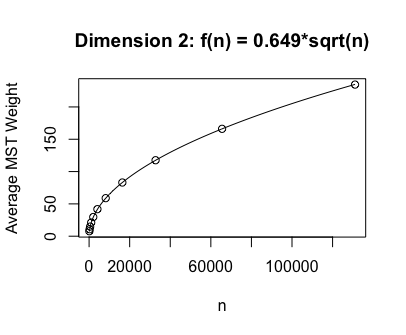
\includegraphics[width=2.27in]{dim2plot}
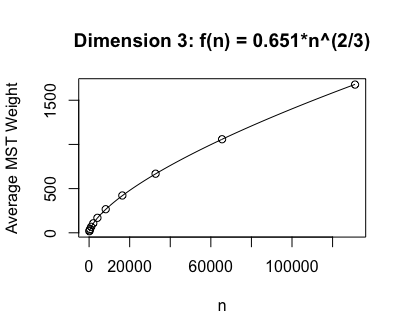
\includegraphics[width=2.27in]{dim3plot}
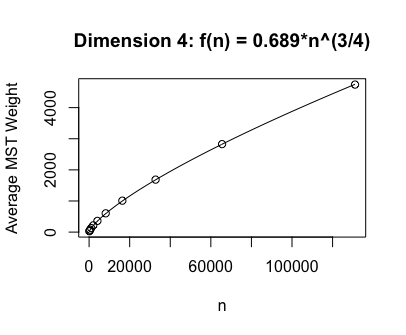
\includegraphics[width=2.27in]{dim4plot}

The growth rate for Euclidean distance-weighted graphs is not surprising. First, we note that this function's second derivative is negative, indicating that greater values of $n$ correspond to a lesser increase in $f(n)$. This makes sense, because increasing the number of vertices while limiting the coordinates of each vertex to a unit square/cube/hypercube results in vertices that are clustered more closely together, decreasing the impact of any additional vertices on total MST weight. Thus, a increase in $n$ will not result in an equally proportional increase in $f(n)$, since new vertices are likely to be closer together to existing vertices.

Second, we also note that as the numbers of dimensions increases, the growth rate of $f(n)$ approaches $O(n)$. Again, this makes sense, because increasing the number of dimensions that each vertex has access to decreases the aforementioned clustering effect; that is, adding additional vertices are less likely to result in a graph that is tightly clustered, since these extra vertices are more likely to be "farther" away from existing vertices.

For the random weights case, we simply model the relationship with a constant, because we noted that values of $f(n)$ appeared to converge to a value of around 1.203 as $n$ increased. The data are plotted below, along with a line representing the average value of $f(n)$.

\begin{center}
	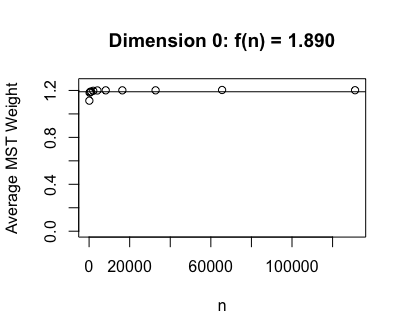
\includegraphics[width=3.4in]{dim0plot}
\end{center}

Intuitively, this result is not surprising, because increasing $n$ here simply adds vertices to a cluster of extremely ``closely-connected'' nodes (if we visualize edge weight as distance), such that adding additional vertices will have less and less impact on the total minimum spanning tree weight as the size of the graph increases (since any additional vertices will exist within this dense ball).

\end{document}